\documentclass{standalone}
\usepackage{tikz}
\usetikzlibrary{patterns, positioning}

\begin{document}
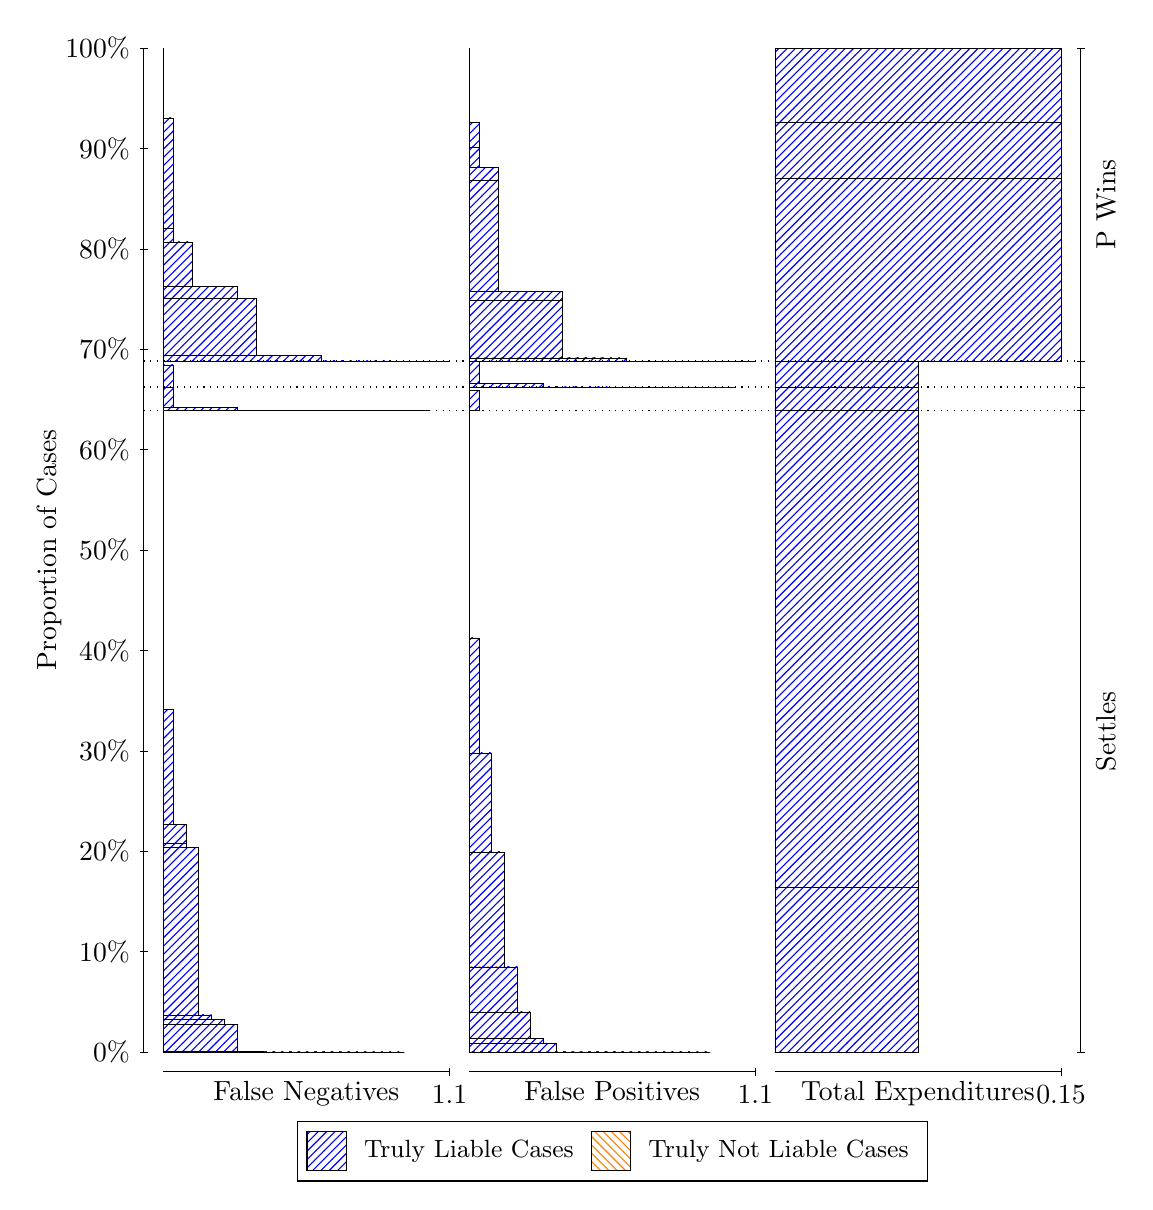
\begin{tikzpicture}
\draw[black, very thin] (1.5,1.75) -- (1.5,14.5);
\node[rotate=90, anchor=center] at (0.3, 8.125) {Proportion of Cases};
\draw[black, very thin] (1.45,1.75) -- (1.55,1.75);
\node[anchor=east] at (1.45, 1.75) {0\%};
\draw[black, very thin] (1.45,3.025) -- (1.55,3.025);
\node[anchor=east] at (1.45, 3.025) {10\%};
\draw[black, very thin] (1.45,4.3) -- (1.55,4.3);
\node[anchor=east] at (1.45, 4.3) {20\%};
\draw[black, very thin] (1.45,5.575) -- (1.55,5.575);
\node[anchor=east] at (1.45, 5.575) {30\%};
\draw[black, very thin] (1.45,6.85) -- (1.55,6.85);
\node[anchor=east] at (1.45, 6.85) {40\%};
\draw[black, very thin] (1.45,8.125) -- (1.55,8.125);
\node[anchor=east] at (1.45, 8.125) {50\%};
\draw[black, very thin] (1.45,9.4) -- (1.55,9.4);
\node[anchor=east] at (1.45, 9.4) {60\%};
\draw[black, very thin] (1.45,10.675) -- (1.55,10.675);
\node[anchor=east] at (1.45, 10.675) {70\%};
\draw[black, very thin] (1.45,11.95) -- (1.55,11.95);
\node[anchor=east] at (1.45, 11.95) {80\%};
\draw[black, very thin] (1.45,13.225) -- (1.55,13.225);
\node[anchor=east] at (1.45, 13.225) {90\%};
\draw[black, very thin] (1.45,14.5) -- (1.55,14.5);
\node[anchor=east] at (1.45, 14.5) {100\%};

\draw[black, very thin] (13.4,1.75) -- (13.4,14.5);
\draw[black, very thin] (13.35,1.75) -- (13.45,1.75);
\node[anchor=west] at (13.35, 1.75) {};
\draw[black, very thin] (13.35,9.8976) -- (13.45,9.8976);
\node[anchor=west] at (13.35, 9.8976) {};
\draw[black, very thin] (13.35,10.195) -- (13.45,10.195);
\node[anchor=west] at (13.35, 10.195) {};
\draw[black, very thin] (13.35,10.525) -- (13.45,10.525);
\node[anchor=west] at (13.35, 10.525) {};
\draw[black, very thin] (13.35,14.5) -- (13.45,14.5);
\node[anchor=west] at (13.35, 14.5) {};

\draw[black, very thin, pattern color=blue, pattern=north east lines] (1.75,1.75) rectangle (4.8118,1.75);
\draw[black, very thin, pattern color=blue, pattern=north east lines] (1.75,1.75) rectangle (4.4852,1.75);
\draw[black, very thin, pattern color=blue, pattern=north east lines] (1.75,1.75) rectangle (4.1586,1.75);
\draw[black, very thin, pattern color=blue, pattern=north east lines] (1.75,1.75) rectangle (3.9953,1.75);
\draw[black, very thin, pattern color=blue, pattern=north east lines] (1.75,1.75) rectangle (3.832,1.75);
\draw[black, very thin, pattern color=blue, pattern=north east lines] (1.75,1.75) rectangle (3.6687,1.75);
\draw[black, very thin, pattern color=blue, pattern=north east lines] (1.75,1.75) rectangle (3.5054,1.7509);
\draw[black, very thin, pattern color=blue, pattern=north east lines] (1.75,1.7509) rectangle (3.3421,1.7509);
\draw[black, very thin, pattern color=blue, pattern=north east lines] (1.75,1.7509) rectangle (3.1788,1.751);
\draw[black, very thin, pattern color=blue, pattern=north east lines] (1.75,1.751) rectangle (3.0155,1.751);
\draw[black, very thin, pattern color=blue, pattern=north east lines] (1.75,1.751) rectangle (3.0155,1.7539);
\draw[black, very thin, pattern color=blue, pattern=north east lines] (1.75,1.7539) rectangle (2.8522,1.7573);
\draw[black, very thin, pattern color=blue, pattern=north east lines] (1.75,1.7573) rectangle (2.689,2.0973);
\draw[black, very thin, pattern color=blue, pattern=north east lines] (1.75,2.0973) rectangle (2.5257,2.163);
\draw[black, very thin, pattern color=blue, pattern=north east lines] (1.75,2.163) rectangle (2.5257,2.163);
\draw[black, very thin, pattern color=blue, pattern=north east lines] (1.75,2.163) rectangle (2.3624,2.2207);
\draw[black, very thin, pattern color=blue, pattern=north east lines] (1.75,2.2207) rectangle (2.1991,2.2207);
\draw[black, very thin, pattern color=blue, pattern=north east lines] (1.75,2.2207) rectangle (2.1991,4.3444);
\draw[black, very thin, pattern color=blue, pattern=north east lines] (1.75,4.3444) rectangle (2.0358,4.3992);
\draw[black, very thin, pattern color=blue, pattern=north east lines] (1.75,4.3992) rectangle (2.0358,4.6381);
\draw[black, very thin, pattern color=blue, pattern=north east lines] (1.75,4.6381) rectangle (1.8725,6.1006);
\draw[black, very thin, pattern color=orange, pattern=north west lines] (1.75,6.1006) rectangle (1.75,6.1006);
\draw[black, very thin, pattern color=blue, pattern=north east lines] (1.75,6.1006) rectangle (1.75,9.8976);
\draw[black, very thin, pattern color=blue, pattern=north east lines] (1.75,9.8976) rectangle (5.1384,9.8976);
\draw[black, very thin, pattern color=blue, pattern=north east lines] (1.75,9.8976) rectangle (4.3219,9.8976);
\draw[black, very thin, pattern color=blue, pattern=north east lines] (1.75,9.8976) rectangle (3.5054,9.8979);
\draw[black, very thin, pattern color=blue, pattern=north east lines] (1.75,9.8979) rectangle (2.689,9.938);
\draw[black, very thin, pattern color=blue, pattern=north east lines] (1.75,9.938) rectangle (1.8725,10.195);
\draw[black, very thin, pattern color=orange, pattern=north west lines] (1.75,10.195) rectangle (1.75,10.195);
\draw[black, very thin, pattern color=blue, pattern=north east lines] (1.75,10.195) rectangle (1.8725,10.475);
\draw[black, very thin, pattern color=orange, pattern=north west lines] (1.75,10.475) rectangle (1.75,10.475);
\draw[black, very thin, pattern color=blue, pattern=north east lines] (1.75,10.475) rectangle (1.75,10.525);
\draw[black, very thin, pattern color=blue, pattern=north east lines] (1.75,10.525) rectangle (5.3833,10.525);
\draw[black, very thin, pattern color=blue, pattern=north east lines] (1.75,10.525) rectangle (4.5669,10.526);
\draw[black, very thin, pattern color=blue, pattern=north east lines] (1.75,10.526) rectangle (4.3219,10.526);
\draw[black, very thin, pattern color=blue, pattern=north east lines] (1.75,10.526) rectangle (3.7504,10.597);
\draw[black, very thin, pattern color=blue, pattern=north east lines] (1.75,10.597) rectangle (3.5054,10.597);
\draw[black, very thin, pattern color=blue, pattern=north east lines] (1.75,10.597) rectangle (2.9339,11.321);
\draw[black, very thin, pattern color=blue, pattern=north east lines] (1.75,11.321) rectangle (2.689,11.47);
\draw[black, very thin, pattern color=blue, pattern=north east lines] (1.75,11.47) rectangle (2.1174,12.038);
\draw[black, very thin, pattern color=blue, pattern=north east lines] (1.75,12.038) rectangle (1.8725,12.21);
\draw[black, very thin, pattern color=blue, pattern=north east lines] (1.75,12.21) rectangle (1.8725,13.612);
\draw[black, very thin, pattern color=orange, pattern=north west lines] (1.75,13.612) rectangle (1.75,13.612);
\draw[black, very thin, pattern color=blue, pattern=north east lines] (1.75,13.612) rectangle (1.75,14.5);
\draw[black, very thin, pattern color=orange, pattern=north west lines] (5.6333,1.75) rectangle (8.6951,1.75);
\draw[black, very thin, pattern color=blue, pattern=north east lines] (5.6333,1.75) rectangle (8.6951,1.75);
\draw[black, very thin, pattern color=orange, pattern=north west lines] (5.6333,1.75) rectangle (8.3685,1.75);
\draw[black, very thin, pattern color=blue, pattern=north east lines] (5.6333,1.75) rectangle (8.3685,1.75);
\draw[black, very thin, pattern color=orange, pattern=north west lines] (5.6333,1.75) rectangle (8.0419,1.75);
\draw[black, very thin, pattern color=blue, pattern=north east lines] (5.6333,1.75) rectangle (8.0419,1.75);
\draw[black, very thin, pattern color=blue, pattern=north east lines] (5.6333,1.75) rectangle (7.8787,1.75);
\draw[black, very thin, pattern color=orange, pattern=north west lines] (5.6333,1.75) rectangle (7.7154,1.75);
\draw[black, very thin, pattern color=blue, pattern=north east lines] (5.6333,1.75) rectangle (7.7154,1.75);
\draw[black, very thin, pattern color=blue, pattern=north east lines] (5.6333,1.75) rectangle (7.5521,1.75);
\draw[black, very thin, pattern color=orange, pattern=north west lines] (5.6333,1.75) rectangle (7.3888,1.75);
\draw[black, very thin, pattern color=blue, pattern=north east lines] (5.6333,1.75) rectangle (7.3888,1.7501);
\draw[black, very thin, pattern color=blue, pattern=north east lines] (5.6333,1.7501) rectangle (7.2255,1.7501);
\draw[black, very thin, pattern color=orange, pattern=north west lines] (5.6333,1.7501) rectangle (7.0622,1.7501);
\draw[black, very thin, pattern color=blue, pattern=north east lines] (5.6333,1.7501) rectangle (7.0622,1.7514);
\draw[black, very thin, pattern color=orange, pattern=north west lines] (5.6333,1.7514) rectangle (7.0622,1.7514);
\draw[black, very thin, pattern color=blue, pattern=north east lines] (5.6333,1.7514) rectangle (7.0622,1.7514);
\draw[black, very thin, pattern color=blue, pattern=north east lines] (5.6333,1.7514) rectangle (6.8989,1.7514);
\draw[black, very thin, pattern color=blue, pattern=north east lines] (5.6333,1.7514) rectangle (6.7356,1.7514);
\draw[black, very thin, pattern color=orange, pattern=north west lines] (5.6333,1.7514) rectangle (6.7356,1.7514);
\draw[black, very thin, pattern color=blue, pattern=north east lines] (5.6333,1.7514) rectangle (6.7356,1.855);
\draw[black, very thin, pattern color=blue, pattern=north east lines] (5.6333,1.855) rectangle (6.5723,1.9208);
\draw[black, very thin, pattern color=orange, pattern=north west lines] (5.6333,1.9208) rectangle (6.409,1.9208);
\draw[black, very thin, pattern color=blue, pattern=north east lines] (5.6333,1.9208) rectangle (6.409,2.2574);
\draw[black, very thin, pattern color=blue, pattern=north east lines] (5.6333,2.2574) rectangle (6.409,2.2594);
\draw[black, very thin, pattern color=blue, pattern=north east lines] (5.6333,2.2594) rectangle (6.2457,2.8305);
\draw[black, very thin, pattern color=blue, pattern=north east lines] (5.6333,2.8305) rectangle (6.2457,2.8305);
\draw[black, very thin, pattern color=orange, pattern=north west lines] (5.6333,2.8305) rectangle (6.0824,2.8305);
\draw[black, very thin, pattern color=blue, pattern=north east lines] (5.6333,2.8305) rectangle (6.0824,4.2911);
\draw[black, very thin, pattern color=blue, pattern=north east lines] (5.6333,4.2911) rectangle (6.0824,4.2916);
\draw[black, very thin, pattern color=blue, pattern=north east lines] (5.6333,4.2916) rectangle (5.9191,4.2916);
\draw[black, very thin, pattern color=blue, pattern=north east lines] (5.6333,4.2916) rectangle (5.9191,5.547);
\draw[black, very thin, pattern color=blue, pattern=north east lines] (5.6333,5.547) rectangle (5.7558,7.0096);
\draw[black, very thin, pattern color=blue, pattern=north east lines] (5.6333,7.0096) rectangle (5.6333,9.8976);
\draw[black, very thin, pattern color=orange, pattern=north west lines] (5.6333,9.8976) rectangle (5.7558,9.8976);
\draw[black, very thin, pattern color=blue, pattern=north east lines] (5.6333,9.8976) rectangle (5.7558,10.155);
\draw[black, very thin, pattern color=blue, pattern=north east lines] (5.6333,10.155) rectangle (5.6333,10.195);
\draw[black, very thin, pattern color=orange, pattern=north west lines] (5.6333,10.195) rectangle (9.0217,10.195);
\draw[black, very thin, pattern color=blue, pattern=north east lines] (5.6333,10.195) rectangle (9.0217,10.195);
\draw[black, very thin, pattern color=blue, pattern=north east lines] (5.6333,10.195) rectangle (8.2052,10.195);
\draw[black, very thin, pattern color=blue, pattern=north east lines] (5.6333,10.195) rectangle (7.3888,10.196);
\draw[black, very thin, pattern color=blue, pattern=north east lines] (5.6333,10.196) rectangle (6.5723,10.245);
\draw[black, very thin, pattern color=blue, pattern=north east lines] (5.6333,10.245) rectangle (5.7558,10.525);
\draw[black, very thin, pattern color=orange, pattern=north west lines] (5.6333,10.525) rectangle (9.2667,10.525);
\draw[black, very thin, pattern color=blue, pattern=north east lines] (5.6333,10.525) rectangle (9.2667,10.525);
\draw[black, very thin, pattern color=orange, pattern=north west lines] (5.6333,10.525) rectangle (8.4502,10.525);
\draw[black, very thin, pattern color=blue, pattern=north east lines] (5.6333,10.525) rectangle (8.4502,10.525);
\draw[black, very thin, pattern color=orange, pattern=north west lines] (5.6333,10.525) rectangle (7.6337,10.525);
\draw[black, very thin, pattern color=blue, pattern=north east lines] (5.6333,10.525) rectangle (7.6337,10.566);
\draw[black, very thin, pattern color=orange, pattern=north west lines] (5.6333,10.566) rectangle (7.3888,10.566);
\draw[black, very thin, pattern color=blue, pattern=north east lines] (5.6333,10.566) rectangle (7.3888,10.566);
\draw[black, very thin, pattern color=blue, pattern=north east lines] (5.6333,10.566) rectangle (6.8172,11.292);
\draw[black, very thin, pattern color=orange, pattern=north west lines] (5.6333,11.292) rectangle (6.8172,11.292);
\draw[black, very thin, pattern color=blue, pattern=north east lines] (5.6333,11.292) rectangle (6.8172,11.412);
\draw[black, very thin, pattern color=orange, pattern=north west lines] (5.6333,11.412) rectangle (6.5723,11.412);
\draw[black, very thin, pattern color=blue, pattern=north east lines] (5.6333,11.412) rectangle (6.5723,11.413);
\draw[black, very thin, pattern color=blue, pattern=north east lines] (5.6333,11.413) rectangle (6.0007,12.815);
\draw[black, very thin, pattern color=blue, pattern=north east lines] (5.6333,12.815) rectangle (6.0007,12.986);
\draw[black, very thin, pattern color=orange, pattern=north west lines] (5.6333,12.986) rectangle (5.7558,12.986);
\draw[black, very thin, pattern color=blue, pattern=north east lines] (5.6333,12.986) rectangle (5.7558,13.245);
\draw[black, very thin, pattern color=blue, pattern=north east lines] (5.6333,13.245) rectangle (5.7558,13.554);
\draw[black, very thin, pattern color=blue, pattern=north east lines] (5.6333,13.554) rectangle (5.6333,14.5);
\draw[black, very thin, pattern color=orange, pattern=north west lines] (9.5167,1.75) rectangle (11.333,1.75);
\draw[black, very thin, pattern color=blue, pattern=north east lines] (9.5167,1.75) rectangle (11.333,3.8416);
\draw[black, very thin, pattern color=orange, pattern=north west lines] (9.5167,3.8416) rectangle (11.333,3.8416);
\draw[black, very thin, pattern color=blue, pattern=north east lines] (9.5167,3.8416) rectangle (11.333,9.8976);
\draw[black, very thin, pattern color=orange, pattern=north west lines] (9.5167,9.8976) rectangle (11.333,9.8976);
\draw[black, very thin, pattern color=blue, pattern=north east lines] (9.5167,9.8976) rectangle (11.333,10.195);
\draw[black, very thin, pattern color=orange, pattern=north west lines] (9.5167,10.195) rectangle (11.333,10.195);
\draw[black, very thin, pattern color=blue, pattern=north east lines] (9.5167,10.195) rectangle (11.333,10.525);
\draw[black, very thin, pattern color=orange, pattern=north west lines] (9.5167,10.525) rectangle (13.15,10.525);
\draw[black, very thin, pattern color=blue, pattern=north east lines] (9.5167,10.525) rectangle (13.15,12.843);
\draw[black, very thin, pattern color=orange, pattern=north west lines] (9.5167,12.843) rectangle (13.15,12.843);
\draw[black, very thin, pattern color=blue, pattern=north east lines] (9.5167,12.843) rectangle (13.15,13.555);
\draw[black, very thin, pattern color=orange, pattern=north west lines] (9.5167,13.555) rectangle (13.15,13.555);
\draw[black, very thin, pattern color=blue, pattern=north east lines] (9.5167,13.555) rectangle (13.15,14.5);
\draw[black, dotted] (1.5,9.8976) -- (13.4,9.8976);
\draw[black, dotted] (1.5,10.195) -- (13.4,10.195);
\draw[black, dotted] (1.5,10.525) -- (13.4,10.525);
\draw[black, very thin] (1.75,1.5) -- (5.3833,1.5);
\node[anchor=north] at (3.5667, 1.5) {False Negatives};
\draw[black, very thin] (5.3833,1.45) -- (5.3833,1.55);
\node[anchor=north] at (5.3833, 1.45) {1.1};

\draw[black, very thin] (5.6333,1.5) -- (9.2667,1.5);
\node[anchor=north] at (7.45, 1.5) {False Positives};
\draw[black, very thin] (9.2667,1.45) -- (9.2667,1.55);
\node[anchor=north] at (9.2667, 1.45) {1.1};

\draw[black, very thin] (9.5167,1.5) -- (13.15,1.5);
\node[anchor=north] at (11.333, 1.5) {Total Expenditures};
\draw[black, very thin] (13.15,1.45) -- (13.15,1.55);
\node[anchor=north] at (13.15, 1.45) {0.15};

\node[black, centered, rotate=90] at (13.72, 5.8238) {Settles};


\node[black, centered, rotate=90] at (13.72, 12.512) {P Wins};

\draw (7.449999999999999,1.5) node[draw=none] (baseCoordinate) {};
\begin{scope}[align=center]
        \matrix[scale=0.5, draw=black, below=0.5cm of baseCoordinate, nodes={draw}, column sep=0.1cm]{
            \node[rectangle, draw, minimum width=0.5cm, minimum height=0.5cm, pattern=north east lines, pattern color=blue] {}; &
            \node[draw=none, font=\small] (B) {Truly Liable Cases}; &
            \node[rectangle, draw, minimum width=0.5cm, minimum height=0.5cm, pattern=north west lines, pattern color=orange] {}; &
            \node[draw=none, font=\small] (B) {Truly Not Liable Cases}; \\
            };
\end{scope}

\end{tikzpicture}
\end{document}